\section{Material and Method}

\begin{figure*}[!htb]
\centering
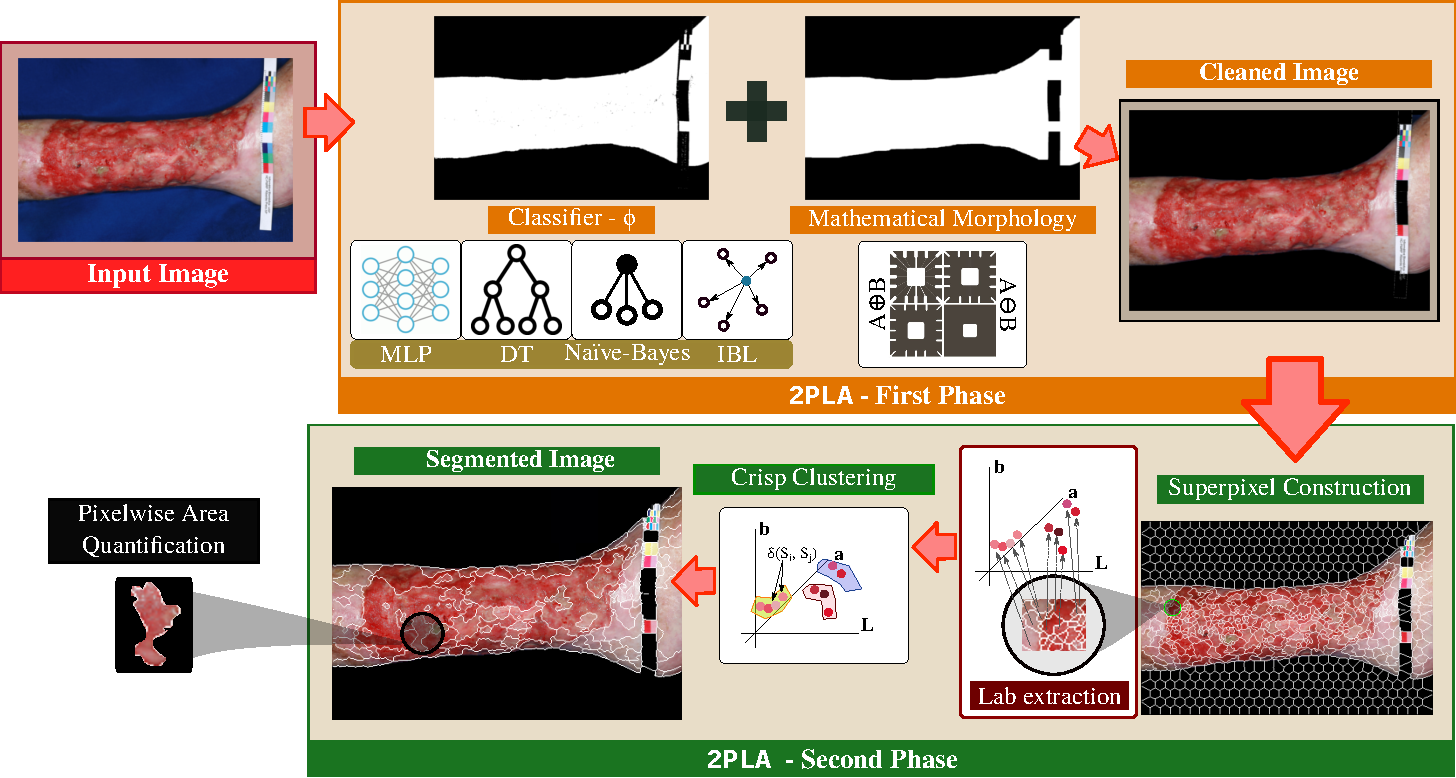
\includegraphics[scale=.66]{figs/pipeline2.pdf}
\caption{Overall \system pipeline.
\system first phase removes background points through pixelwise classification and mathematical morphology.
Cleaned images are divided into superpixels further represented in the $Lab$ color space.
\system second phase applies a crisp cluster approach for grouping similar superpixels, and joint regions can be masked back into the input image. 
Segmented tissues are quantified regarding the number of inner pixels.}
\label{fig:system}
\end{figure*}
This section describes a two-phase method for chronic wound segmentation as well as the ulcer dataset we employed for the tuning and evaluation of our approach.\\

\noindent
\textbf{Data source.} 
We consider data source \dataset~\cite{Pereyra2014} in the design and evaluation of our proposal.
Such an image set includes $217$ photographies of venous and arterial ulcers in lower limbs with varying sizes and distinct healing stages regarding patients with different skin colors, age, and treatments.
Blue and white cloths were used to emphasize the contrast between the background and the patients' skin, and photos were taken with the same camera, angle and distance.
Color patches and rulers were also included in the images to facilitate color normalization and area calibration.
We asked experts to provide a manual segmentation of $40$ representative \dataset images to be used as the \textit{ground-truth} in all subsequent evaluations.
As a result, millions of pixels were labeled as ``background'' and ``skin'', while regions of interest were divided into ``border'' and ``interior'' tissues, which include parts of granulation, fibrin, and necrosis.\\


\noindent
\textbf{\system pipeline.} 
Our proposal, named \system, can be seen as a sequential pipeline for chronic wounds segmentation\footnote{\url{github.com/sswellington/2PLA}}.
The main idea is removing background points eases the similarity-based clustering of superpixels with well-defined borders.
Figure~\ref{fig:system} describes \system pipeline according to a sample image from \dataset.
In \system first phase, pixels of class ``skin'' are selected as relevant, whereas ``background'' pixels are dismissed.
Potential misclassifications of pixels at lower limb borders are rectified by the following morphological operators 
\textit{(i)}~median filter, 
\textit{(ii)}~Otsu binarization of skin pixels, and 
\textit{(iii)}~opening.
%The morphological structuring element perimeter is set to $1\%$ of the input image perimeter.
Cleaned images are fed to \system  divide-and-conquer second phase, in which background-free images are divided into superpixels by SLIC construction algorithm, while superpixel average values are extracted into the $Lab$ color space.
Next, DBSCAN is employed for the grouping of extracted points according to their similarity and density.
Clustered superpixels are joint into a single piece of tissue, which is quantified regarding the number of inner pixels.

Algorithm~\ref{alg:1} relies on a set of parameters for the implementation of \system pipeline.
Parameter $K_p$ defines the number of constructed superpixels, and parameter $\phi$ is a trained classifier for the labeling of skin pixels, whereas parameters $\delta$ and $\xi$ are DBSCAN settings that define how the similarity between two superpixels is measured and maximum dissimilarity threshold, respectively.
Accordingly, the tuning of \system depends on setting suitable values for Algorithm~\ref{alg:1} parameters.
\vspace{-7px}

\SetKwFunction{slic}{SLIC}
\SetKwFunction{dbscan}{DBSCAN}
\SetKwFunction{morph}{MATH\_MORPHOLOGY}
\SetKwInOut{Input}{Input}
\SetKwInOut{Output}{Output}
\begin{algorithm}[!htb]
\small
\hrulefill

 \Input{Image $I$, metric $\delta$, similarity threshold $\xi$, number of superpixels $K_p$, and trained classifier $\phi$.}
 \Output{Segmented tissues within and around the ulcer.}
 \vspace{-4px}
 \hrulefill
 
 $P_a \leftarrow \langle 0, 0, 0\rangle$\;
\tcc{Discards points of no-interest}
\For{$P_i \in I$}{
    \If{$\phi(P_i) \neq$ ``skin''}{
        $P_i \leftarrow P_a$\;
    }
} %For
$I \leftarrow$ \morph{$I$}\;
$\mathcal{S} \leftarrow$ \slic{$I$, $K_p$}\;
\tcc{Discards $S \in \mathcal{S}$ whenever $\varepsilon(\bar{P_S}) = \varepsilon(P_a)$}
$\mathcal{S'} \leftarrow$ \dbscan{$\mathcal{S}, \delta, \xi, P_a$}\;
\Return $\mathcal{S'}$ masked on $I$\;
 \vspace{-4px}
\hrulefill
 \vspace{2px}
\caption{\system implementation.}
\label{alg:1}
\end{algorithm}
\vspace{-12px}



